\def\pgfsysdriver{pgfsys-dvipdfm.def}
%\documentclass[aspectratio=1610]{beamer}
\documentclass{beamer}
\usetheme[progressbar=head, titleformat=allcaps,block=fill]{metropolis}
\usepackage[orientation=landscape,size=custom,width=16,height=11.15,scale=.5,debug]{beamerposter}

%%% PACKAGES AND INPUTS
\usepackage{pgfopts}
\usepackage{pgfpages}
\usepackage{graphicx}
\usepackage{xcolor}
\usepackage{tikz}
\usetikzlibrary{3d,hyperref}
\usepackage{verbatim}
\usepackage{comment}
%\input{153controls}
\usepackage{pgfplots}
\usepackage{linalgjh}

\usepackage{multicol}


%%% POLAR SETUP
\usepgfplotslibrary{polar}
\pgfplotsset{compat=1.10}
\pgfplotsset{mypolarplot/.style={%
  clip=false, % needed for double line (last \addplot command)
  domain=0:360, % plot full cycle
  samples=180, % number of samples; can be locally adjusted
  grid=both, % display major and minor grids
  major grid style={black}, 
  minor x tick num=3, % 3 minor x ticks between majors
  minor y tick num=1, % 1 minor y tick between majors
  xtick={0,45,...,359},
  xticklabels={%
    $0$,
    $\frac{ \pi}{4}$,
    $\frac{ \pi}{2}$,
    $\frac{3\pi}{4}$,
    $\pi$,
    $\frac{5\pi}{4}$,
    $\frac{3\pi}{2}$,
    $\frac{7\pi}{4}$
  },
  yticklabel style={anchor=north}, % move label position
}}

%%%% COLORS
\definecolor{gold}{HTML}{ffb81c}
\definecolor{heypurple}{HTML}{6B0FFF}
\definecolor{darkgold}{HTML}{5A440D}
\definecolor{darkblue}{HTML}{00268D}
\definecolor{proof}{RGB}{55,54,172}
\definecolor{nicegreen}{RGB}{0,127,35}
\definecolor{remgrey}{RGB}{179,179,179}
\definecolor{Purple}{HTML}{3C0940}
\definecolor{darkgreen}{HTML}{214009}
\definecolor{Orange}{HTML}{7F2000}
\definecolor{Blue}{HTML}{003E78}
\definecolor{Gold}{HTML}{FFCB0A}
\definecolor{gvsublue1}{HTML}{0065a4}
\definecolor{gvsublue2}{HTML}{88B3DA}
\definecolor{unlred}{HTML}{D00000}
\definecolor{DordtGrey}{RGB}{127,127,127}
\definecolor{newred}{HTML}{85140D}
\definecolor{msugreen}{HTML}{023328}
\definecolor{seafoam}{HTML}{127F67}
\definecolor{mnmaroon}{HTML}{790018}
\definecolor{mngold}{HTML}{FFD75F}
\definecolor{fallfoliage}{HTML}{763626}
\definecolor{stone}{HTML}{336B87}
\definecolor{shadow}{HTML}{2A3132}
\definecolor{grass}{HTML}{486B00}
\definecolor{thundercloud}{HTML}{505160}
\definecolor{meadow}{HTML}{598234}
\definecolor{ink}{HTML}{20232A}
\definecolor{rubyred}{HTML}{A01D26}
\definecolor{stormysea}{HTML}{335252}
\definecolor{rust}{HTML}{AA4B41}
\definecolor{forest}{HTML}{1E434C}
\definecolor{crimson}{HTML}{8D230F}
\definecolor{vtgold}{HTML}{C99E10}
\definecolor{vtrust}{HTML}{9B4F0F}

%%%% BEAMER THEMES AND OPTIONS
%\usetheme[progressbar=head,block=fill]{metropolis}
%\setbeameroption{show notes on second screen}
%\metroset{titleformat=smallcaps,block=transparent}
%\usecolortheme{owl}
\setbeamercolor{progress bar}{fg=heypurple,bg=heypurple!30}
\setsansfont[BoldFont={Graphik Semibold},Numbers={Produkt}]{Graphik}


%%% Dordt
%\setbeamercolor{alerted text}{fg=gold}
%\setbeamercolor{normal text}{fg=black}
%%%\setbeamercolor{block}{transparent}
%%%\setbeamercolor{sectionpage}{bg=white}
%%%\setbeamercolor{titleformatpage}{bg=white}
%\setbeamercolor{frametitle}{fg=gold,bg=black!2}
%%%%% GREEN OPTION
%%%\setbeamercolor{alerted text}{fg=seafoam} 
%%%\setbeamercolor{frametitle}{bg=msugreen}



%%% Purple
\setbeamercolor{alerted text}{fg=heypurple}
\setbeamercolor{normal text}{fg=black}
%%\setbeamercolor{block}{transparent}
%%\setbeamercolor{sectionpage}{bg=white}
%%\setbeamercolor{titleformatpage}{bg=white}
\setbeamercolor{frametitle}{fg=heypurple,bg=black!2}
%%%% GREEN OPTION
%%\setbeamercolor{alerted text}{fg=seafoam} 
%%\setbeamercolor{frametitle}{bg=msugreen}




%%% UMICH OPTION
%\setbeamercolor{alerted text}{fg=gold}
%\setbeamercolor{frametitle}{bg=Blue}

%%% MN OPTION
%\setbeamercolor{alerted text}{fg=gold}
%\setbeamercolor{frametitle}{bg=mnmaroon}

%%% FALL MOUNTAIN
%\setbeamercolor{alerted text}{fg=fallfoliage}
%\setbeamercolor{frametitle}{bg=shadow}
%\setbeamercolor{alerted text}{fg=stone}
%\setbeamercolor{alerted text}{fg=grass}

%%% ICELAND
%\setbeamercolor{alerted text}{fg=meadow}
%\setbeamercolor{frametitle}{bg=thundercloud}


%%% VERMONT
%\setbeamercolor{alerted text}{fg=crimson}
%\setbeamercolor{alerted text}{fg=vtrust}
%\setbeamercolor{frametitle}{bg=thundercloud}


%%% INDUSTRIAL
%\setbeamercolor{alerted text}{fg=rubyred}
%\setbeamercolor{frametitle}{bg=ink}

%%% SAN FRANCISCO
%\setbeamercolor{alerted text}{fg=rust}
%\setbeamercolor{frametitle}{bg=stormysea}


%%%% MACROS
\def\rem#1{{\hfill \textit{\tiny {\color{remgrey} {#1}}}}}
\def\h#1{\alert{#1}}
\def\C{{\mathbb C}}
\def\Z{{\mathbb Z}}
\def\F{{\mathbb F}}
\def\bF{{\mathbb F}}
\def\Q{{\mathbb Q}}
\def\R{{\mathbb R}}
\def\P{{\mathbb P}}
\def\A{{\mathbb A}}
\def\N{{\mathbb N}}
\def\i{\mathbf i}}
\def\j{\mathbf j}}
\def\k{\mathbf k}}
\def\proj{{\text{proj}}}
\def\comp{{\text{comp}}}
\def\set#1{\left\{ {#1} \right\}}
\def\setof#1#2{{\left\{#1\,:\,#2\right\}}}


%%%% ENVIRONMENTS
\newenvironment{proof-idea}{\noindent{\alert{Proof Idea.}}\hspace*{1em}}{\qed\bigskip\\}
\newtheorem{conj}{Conjecture}
\newtheorem{prop}{Proposition}
\newtheorem{cor}{Corollary}
\newtheorem{defn}{Definition}
\newtheorem{question}{Question}
\newtheorem{goal}{Goal}

\usepackage{cancel}
\newcommand\lheq{\mathrel{\overset{\makebox[0pt]{\mbox{\normalfont\tiny\sffamily \alert{L'H}}}}{=}}}

\title{\S 4.2: Determining Distance Traveled from Velocity}
%\subtitle{Welcome!}
\author{Dr.\ Mike Janssen}
\date{April 2, 2021}

\begin{document}



\frame{\titlepage}








\frame{
	\frametitle{Announcements}
	
	\begin{itemize}

	
	
\end{itemize}

}






\frame{
	\frametitle{Preview Activity Discussion}
	
	

}


\frame{
	\frametitle{First: Sigma Notation}
	
	Intent: develop a compact way of writing a sum of many terms.\pause
	
	Examples:
	
	\[
		$\sum_{k=1}^{100} k = 1 + 2 + 3 + \cdots + 99 + 100
	\]\pause
	
	\[
		$\sum_{n=1}^{50} \frac{n(n+1)}{2} = \frac{1(1+1)}{2} + \frac{2(2+1)}{2} + \cdots + \frac{49(49+1)}{2} + \frac{50(50+1)}{2}
	\]

}

\frame{
	\frametitle{Activity 4.2.2}

}

\section{Riemann Sums}

\frame{
	\frametitle{Bernhard Riemann}
	
\begin{minipage}[b]{0.45\linewidth}
\begin{itemize}
	\item 1826-1866
	\item Son of a German Lutheran pastor; saw mathematics as a service to God
	\item Riemannian geometry is the foundation of general relativity
	\item First to suggest dimensions greater than 3 or 4 to describe Creation
	\item Riemann Hypothesis -- most famous unsolved math problem
\end{itemize}
\end{minipage}
\hspace{0.5cm}
\begin{minipage}[b]{0.45\linewidth}
\centering
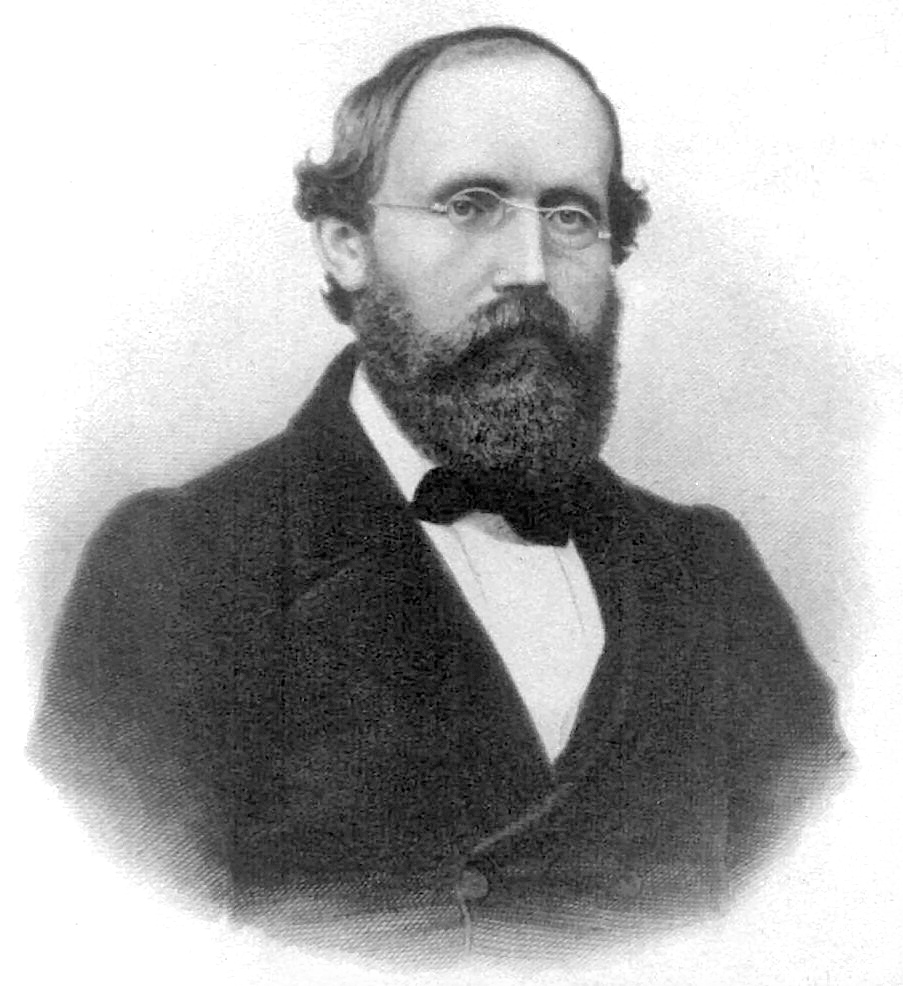
\includegraphics[width=\textwidth]{img/Georg_Friedrich_Bernhard_Riemann.jpeg}
\end{minipage}

}

\frame{
	\frametitle{Goal: Calculate the area under a curve}
	
	Why? \pause
	
	\textbf{Create} an approximation via rectangles.
	
	\pause
	
	Suppose we want to approximate the area under a general (positive) curve given by $y = f(x)$ on the interval $[a,b]$. How do we start? \rem{equal width}

\vspace{2in}
}

\frame{
	\frametitle{Three Approximations}
	
	\begin{itemize}
	\item Left Riemann sum: $L_n = \sum\limits_{i=0}^{n-1} f(x_i) \Delta x$\pause
	\item Right Riemann sum: $R_n = \sum\limits_{i=1}^n f(x_i)\Delta x$\pause
	\item Middle Riemann sum: $M_n = \sum\limits_{i=1}^n f(\overline{x}_i)\Delta x$, where $\overline{x}_i = \frac{x_i + x_{i+1}}{2}$\pause
\end{itemize}

Another option: choose random points in the subintervals. This is more useful for theoretical discussions/proofs, while the above formulae are more useful in practice.

}

\frame{
	\frametitle{Activity 4.2.3}
	
	Helpful: The applet at {\tt https://www.gvsu.edu/s/a9}
	
	\vspace{5in}

}

\frame{
	\frametitle{What if the function is negative?}
	
\begin{center}
		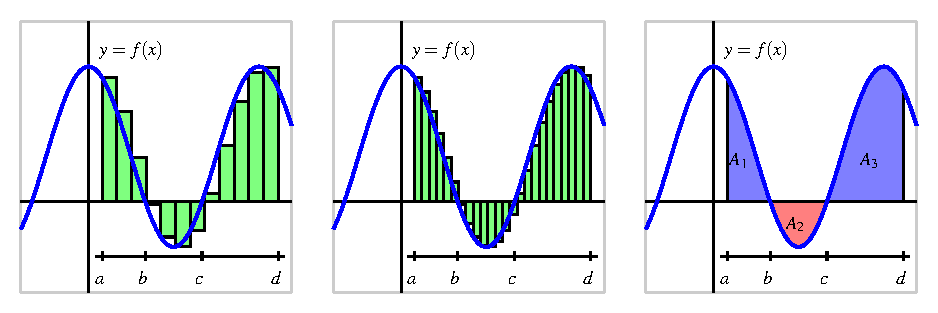
\includegraphics[width=5in]{img/4_2_NegF-eps-converted-to.pdf}
	\end{center}
	
	\pause
	
	This is the \textbf{net signed area bounded by $f$ over the interval $[a,d]$}.

}

\frame{
	\frametitle{Activity 4.2.4}

}

\frame[standout]{

\begin{center}
		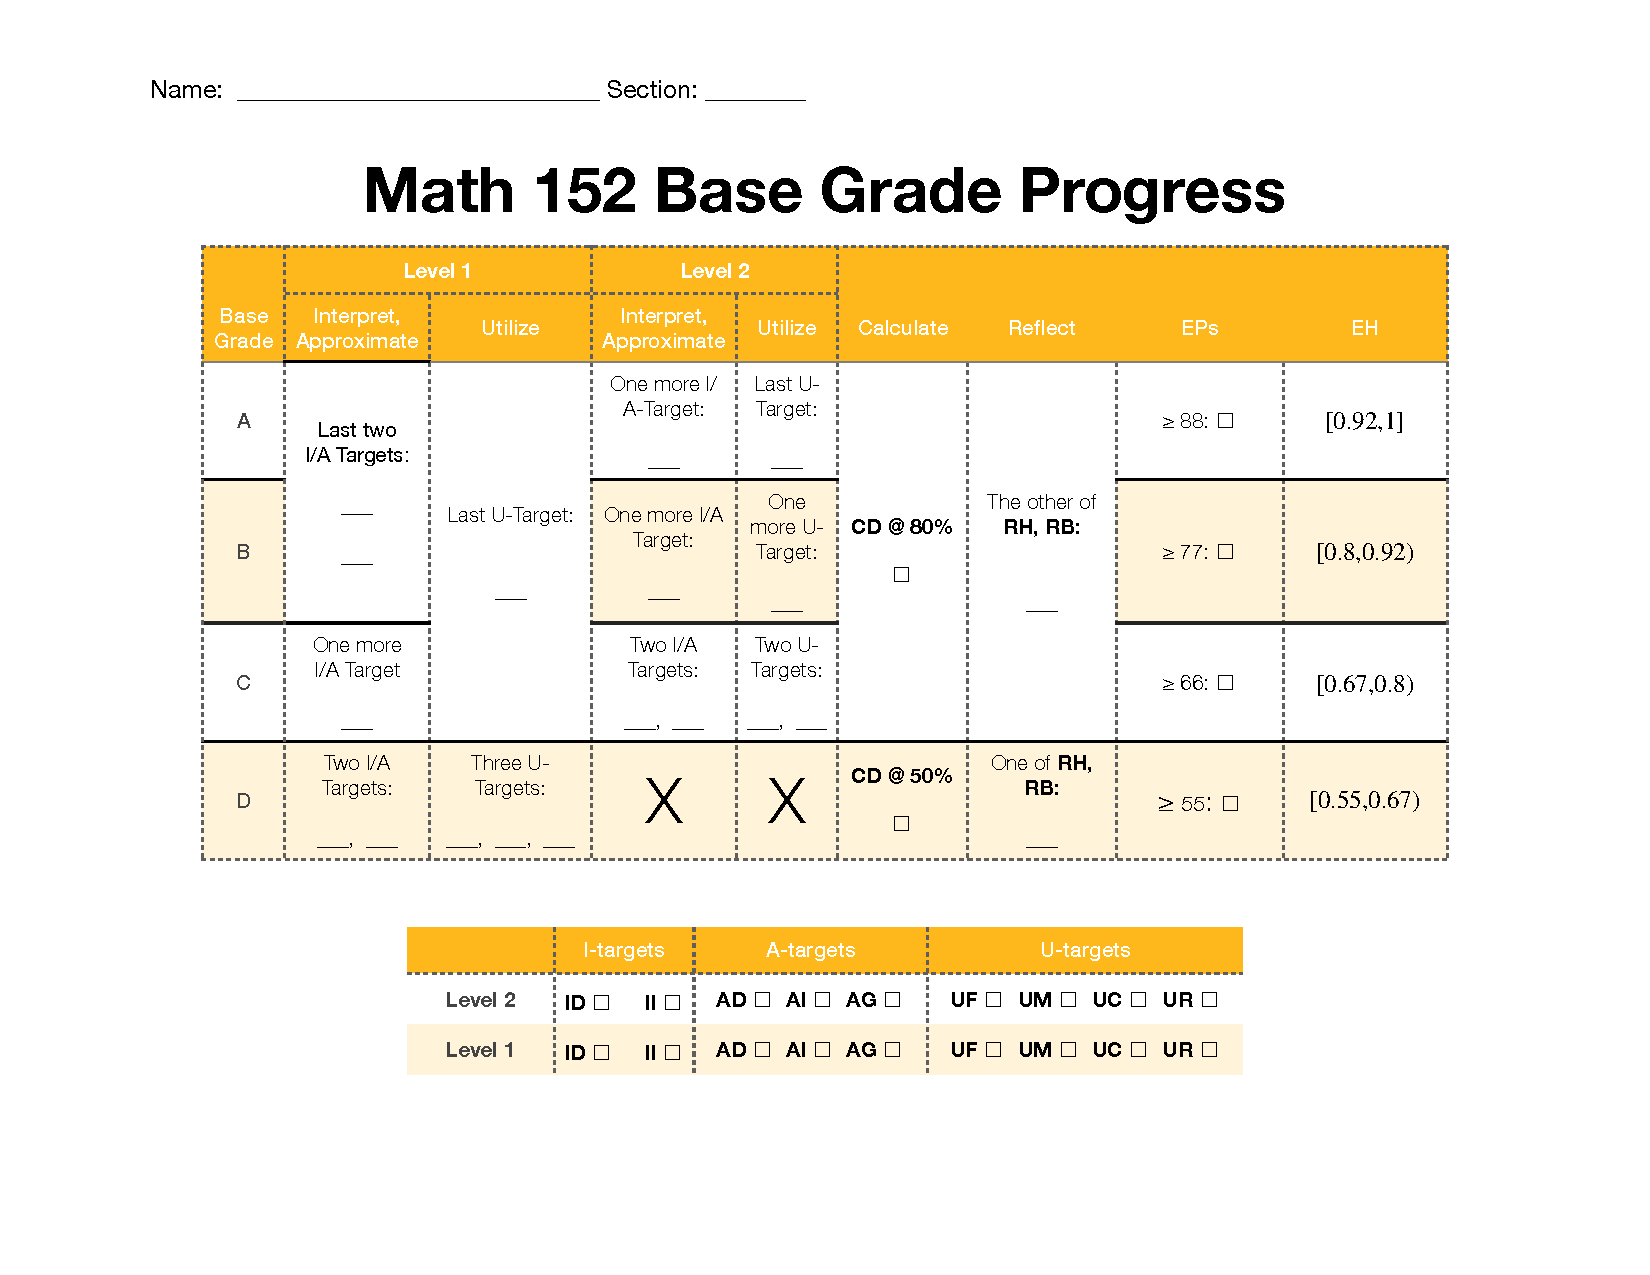
\includegraphics[width=\textwidth]{./img/M152_GradeTracker.pdf}
	\end{center}
}



\end{document}